\section{Design}
\label{sec:design}

Here we present \system{}.  First, we give an overview of the system, and 
then we describe in more detail how content is published, updated, and retrieved.

\subsection{Architecture Overview}
There are four main components in \system{}: 1) origin server, 2) CDN, 3) client, 
and 4) proxy.  The origin server can publish content by first obfuscating the 
content and the content identifier (such as the URL).  This obfuscated data is cached by the CDN 
provider.  A client can request a web page by using one of the proxies associated 
with \system{}.  The proxy re-writes the request such that the request reflects the 
obfuscated content identifier and forwards it onto the CDN.  The CDN locates the 
correct obfuscated content and returns it to the proxy, which un-obfuscates it and
returns it to the client.  The CDN never sees plaintext content or plaintext content 
identifiers and it never sees which client is sending a request.

%\subsection{Obfuscating Content}

%\subsection{Protections Provided by Proxies}

\subsection{Publishing Content}
In order to publish content such that the CDN never sees the content, the publisher 
must first obfuscate her content.  There are two primary steps to publish content: 1) 
obfuscate the data and identifier, and 2) push content to the CDN provider's cache.\footnote{Most CDNs
allow the publisher to decide on a push or pull model, but this makes no difference in our 
system design.}  Figure \ref{fig:publish1} shows the steps taken when publishing content.

\begin{figure}[t]
\centering
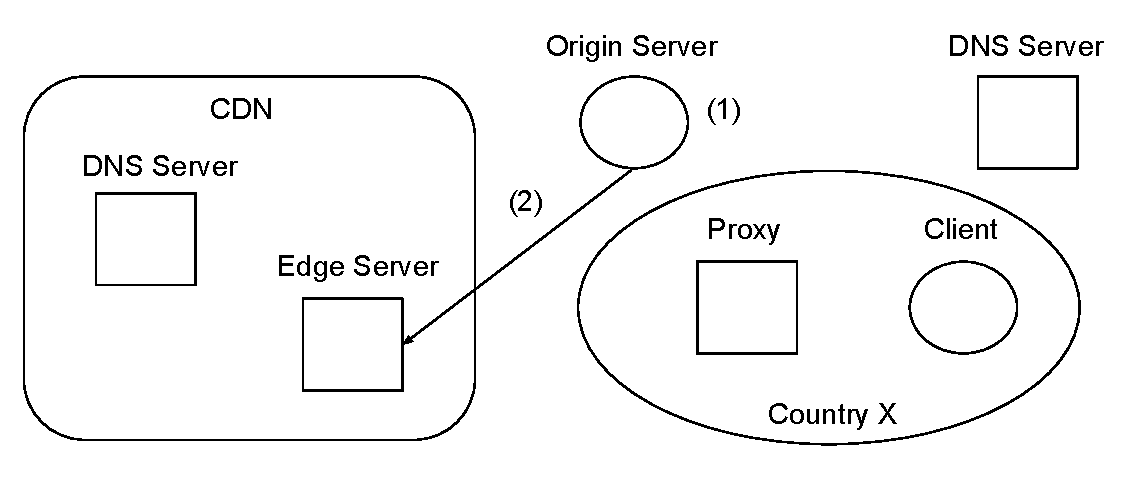
\includegraphics[width=.5\textwidth]{publishing}
\caption{Steps taken to publish content using \system{}.}
\label{fig:publish1}
\end{figure}

The most important step in content publishing is obfuscating the data.  We assume that the origin 
server already has a public and private key pair, as well as a certificate.  To obfuscate the data 
the origin server will need to generate n shared keys, where n should be between 1 and the number of 
proxies.  We reason about the security of different values of n in Section \ref{sec:analysis}.  

Once all keys are established, the publisher must first pad the content to the same size for some 
range of original content sizes (i.e., if content is between length x and y, then pad it to length 
z).  This content padding is done to hide the original content's length, as it may be identifiable 
simply by it's length.  After content is padded, then the content is divided into fixed size blocks and padded to 
some standard length.  Then for each shared key k, each block is encrypted using the shared key, 
such that there are n sets of encrypted blocks.  A visualization of this is shown in Figure \ref{fig:encrypt}.  
As long as the CDN does not have access to any of the n shared keys, then the CDN cannot see what content 
it is caching.  

Now that the content is obfuscated, the publisher must also obfuscate the content's identifier --- usually 
a URL.  To do so, she encrypts the URL with the n shared keys (separately), and then takes a hash of the 
encrypted URL.  She must first encrypt the URL, otherwise an attacker can simply check if the content is 
what he thinks it is by hashing the URL of his guess and checking whether or not it matches.  Since the attacker 
does not know any of the n shared keys, if he hashes a URL, it will never match identifier he's trying to guess.  

Once the identifier and the content are obfuscated n times (with n keys), it can be pushed to the 
CDN.  To increase reliability, performance, and availability, the publisher can push the content to 
multiple CDNs; a publisher can use something like Cedexis~\cite{cedexis} to load balance between 
CDNs.  We discuss the use of multiple CDNs more in Section \ref{sec:partial} on \system{} in 
partial deployment.  Note that each proxy will only be able to fetch a specific replica of the content, that is a 
specific \{content\}$_{kn}$ for the n$^{th}$ shared key that it holds.  We discuss the security and performance trade offs 
associated with differing numbers of shared keys and proxies in Sections \ref{sec:analysis} and \ref{sec:performance}.

\begin{figure}
\centering
   \begin{subfigure}[b]{0.45\textwidth}
   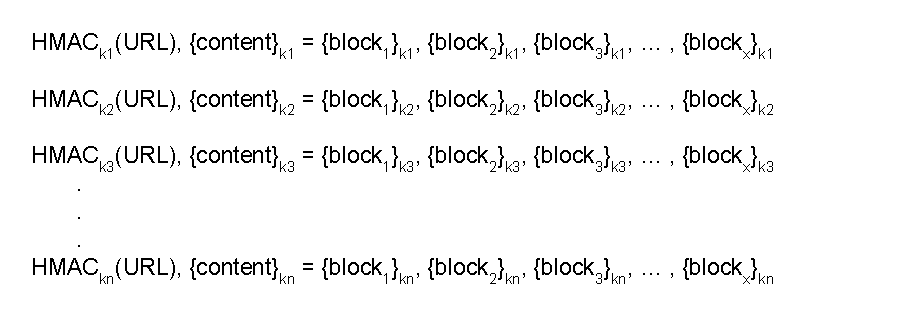
\includegraphics[width=1\linewidth]{encrypt}
   \caption{Multiple copies of the content on the origin server, each encrypted with a different key.}
   \label{fig:encrypt} 
\end{subfigure}

\begin{subfigure}[b]{0.45\textwidth}
   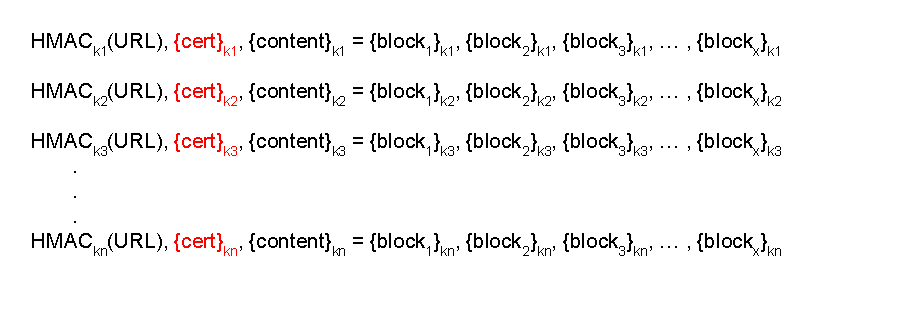
\includegraphics[width=1\linewidth]{https_encrypt}
   \caption{For HTTPS requests, the client must also verify the associated certificate.  Therefore, the 
publisher must also encrypt her certificate (highlighted in red) and push it to the CDN.}
   \label{fig:https_encrypt}
\end{subfigure}

\caption{The obfuscated content, identifier, and certificate that a publisher must 
generate before distributing it to the CDN.}
\end{figure}

\subsection{Updating Content}
For a content publisher to update content, she must follow similar steps as described in the previous subsection.  
Once she has updated the content on her origin server, she must obfuscate it using the same steps: 1) padding the 
original content length, 2) divide the content into fixed size blocks, and 3) encrypt n copies of the content blocks 
with each of the shared keys.  Because she is updating the content (as opposed to creating new content), the 
obfuscated identifier will remain the same (the hash of the URL after it has been encrypted with the shared keys).  She must 
retain a copy of the obfuscated old content until after the new content has been updated on the CDN; this is to prove 
that the old content owner is the same as the new content owner.  Only the origin and the proxy, both of which are 
outside the CDN, know the old obfuscated content, so an attacker cannot update the content that belongs to 
a legitimate publisher.  The publisher must present the old obfuscated content to the CDN in order to also push 
her new obfuscated content to the CDN.  

\subsection{Retrieving Content}
\label{sec:retrieve}
The steps taken for an end-user to retrieve a web page that has been cached by \system{} are shown in Figure \ref{fig:retrieve}.  
The end-user must first configure her browser to use an \system{}-designated proxy.  A client could be assigned to a 
specific proxy, and configure her browser to use the single proxy.  To provide more mixing than the proxy already provides, 
the proxy that is used could be selected based 
on a Proxy Auto Configuration (PAC) file.  Then, once she sends a request for a 
web page, it goes to the proxy via a TLS connection.\footnote{Comment: Add blinding here such that client1's request for foo.com and 
client2's request for foo.com looks different as it goes from the client to the proxy.  So the proxy must be able to un-blind 
the request.}  The proxy then resolves the domain using it's local resolver, which will 
redirect it to the CDN's DNS resolver (as discussed in Section \ref{sec:background}). 

\begin{figure*}[t]
\centering
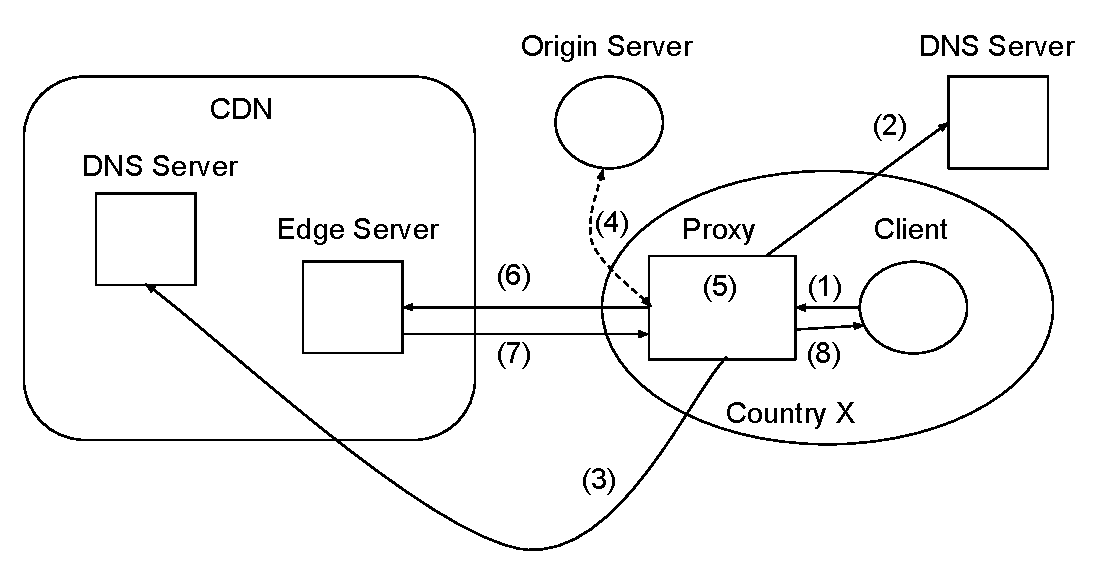
\includegraphics[width=.75\textwidth]{retrieving}
\caption{Steps taken to retrieve a web page using \system{}.}
\label{fig:retrieve}
\end{figure*}

In order for the proxy to generate the obfuscated identifier to query the edge server for the correct content, 
it must have one of the n shared keys that the origin server generated and obfuscated the content and identifier 
with.  The origin server publishes the shared key encrypted with the proxy's public key\footnote{Additionally, the origin server 
can learn the proxy's public key via DNS as well; for example, the proxy can publish it's public key in the DNS SRV record.} in the DNS SRV record; therefore, 
when the proxy sends a DNS request to the origin server's authoritative DNS server, it will receive the the encrypted shared 
key, which it can decrypt with it's private key.  

Now that the proxy has obtained a shared key from the origin server, it can generate the obfuscated content identifier based 
on the request the client sent.  It encrypts the URL with the shared key, and then hashes the encrypted result.  The proxy then 
sends the (obfuscated) request to the edge server, where the CDN locates the content associated with the identifier.  The CDN returns 
the associated obfuscated content, which we recall is the fixed size blocks encrypted with the same shared key that the identifier was 
obfuscated with.  The proxy can decrypt the content blocks with the shared key from the origin server, assemble the blocks, and strip any 
added padding, to reconstruct the original content.\footnote{Comment: Proxy can cache content in times of flash crowd to minimize correlation attacks if a provider has encrypted and unencrypted content on the same CDN.  This raises the issue of charges for the origin (the CDN can’t charge as much if edge servers don’t see as many requests for the origin) --- RFC 2227 describes a solution for this~\cite{rfc2227}.}  Finally, the proxy returns the content to the client over TLS.  

\subsection{HTTPS}
As mentioned in Section \ref{sec:background} it is common practice for CDNs to terminate TLS sessions on behalf of the origin 
server.  CDNs typically perform some types of operations on decrypted content, such as minifying and HTTPS rewrites~\cite{levy2015stickler}.  The fact 
that CDNs terminate TLS sessions puts content integrity into questions, but this is out of the scope of this work, and we are 
primarily concerned with obfuscating the content.  If the CDN is able to access decrypted content, then \system{} does not 
achieve the goals outlined in Section \ref{sec:goals}.  \system{} handles HTTPS requests with a few simple additional steps.

When a content publisher prepares her content to be pushed to the CDN, she has to obfuscate the content and the content identifier (i.e., the 
URL).  If she support HTTPS, then she must also obfuscate her certificate in the same manner; she encrypts the certificate with each shared 
key.  This is shown in Figure \ref{fig:https_encrypt}.  In this case, her content, her content identifier, and her certificate are all cached 
by the CDN, but the CDN does not know the corresponding content or URL.  

When a client sends an HTTPS request, it gets rewritten at the proxy according to the steps in Section \ref{sec:retrieve}.  Once the proxy sends the 
correct request to the CDN, the CDN will return the encrypted content, identifier, and certificate.  The proxy can then decrypt 
the certificate and validate it.  If the certificate is valid, then everything proceeds as described before.  If the certificate is 
not valid, then the proxy drops the data.  One reason that the certificate may not be valid is because it has expired, and when 
this happens, the content publisher should push a new certificate to the CDN to replace the old one.

\subsection{Partial Deployment}
\label{sec:partial}
\system{} should be partially deployable in the sense that if only some of the content publishers participate or only some of the CDNs participate, then 
the system should still provide protections.  We have two different partial deployment plans, and both provide protections for those 
publishers, CDNs, and clients that use \system{}. 

{\bf Plan 1.}
One option for deploying \system{} is to ensure there is some set S of content publishers the participate fully in the 
system.  These publishers obfuscate their content, identifiers, and certificates, and most importantly, only have 
obfuscated data stored on the CDNs cache nodes.  Recall that there are n shared keys, resulting in n replicas of the 
content that {\it appear} to the CDN as different content (because each replica is encrypted with a different key).  This 
allows the minimum set of publishers S to be relatively small.  We discuss the security tradeoffs with different 
values of S in Section \ref{sec:analysis}.  This partial deployment plan protects the set of content publishers S and it 
partially protects the privacy of the clients accessing the content created by the set of publishers S.  It does not 
protect the clients' privacy as completely as full participation of all publishers in \system{} because the CDN can 
still view cross site browsing patterns among the publishers that are not participating. It is important to note though, that 
because the clients are behind proxies, the CDN cannot individually identify users.  The CDN can attribute requests to proxies, but 
not to clients.  

{\bf Plan 2.} 
It is reasonable to believe that some content publishers are skeptical of \system{} and prioritize performance 
and availability.  Therefore, they should have the option to gradually move towards full participation by pushing 
both encrypted and plaintext content to the CDN.  In this partial deployment plan, we see some set of publishers 
fully participating with only encrypted content, some other set of publishers partially participating with both 
encrypted and plaintext content, and some last set of publishers that are not participating.  Unfortunately, if 
a publisher has both encrypted and plaintext content at a cache node, and some event causes a flashcrowd --- 
the CDN sees a significantly larger spike in accesses to certain content --- then the CDN can correlate the access 
spike on encrypted and plaintext content for the same publisher.  In order to prevent this deanonymization of the 
content publisher, we can utilize multiple CDNs.  The publisher can spread replicas over different CDNs such that 
the encrypted replicas are on one CDN and the plaintext replicas are on a different CDN.  In this case the publisher 
is not susceptible to flashcrowds correlations and can still partially join the system.

\subsection{Optimizations}
While there are some optimizations that CDNs typically perform today that would not be possible with \system{}, the architecture 
of \system{} allows for new optimizations that are not possible in existing CDNs.  Here we first outline some ways in which \system{} 
can be optimized in terms of performance, and then we point out what performance enhancements CDNs would not be able to do with 
\system{}.

{\bf Pre-Fetch DNS Responses.} One way to increase the performance of \system{} is to pre-fetch DNS responses at 
the proxies.  This would allow the proxy to serve each client request faster because it would not have to send 
as many DNS requests.  Pre-fetching DNS responses would not take up a large amount of space, but it also 
would not be a complete set of all DNS responses.  Additionally, if the content is moved between cache nodes 
at the CDN, then DNS response must also change; therefore, the pre-fetched DNS responses should have a 
lifetime that is shorter than the lifetime of the content on a cache node.

{\bf Load Balance Proxy Selection.} As the proxy performs a number of operations on the client's behalf, it 
runs into the possibility of being overloaded.  With \system{}, a client can be redirected to different 
proxies based on load; this can be implemented with a PAC file, which allows 
a client to access different proxies for different domains.  In addition to being a performance benefit, 
this could also prevent a country from blocking the set of proxies that all of the country's citizens use; if 
this occurs, then the citizens can be redirected to a different proxy.   

On the other hand, CDNs become more limited in some of their actions when following \system{}'s design.  For example, 
many CDNs perform HTTPS re-writes on content that they cache, but this can only be done if the CDN has access to the 
decrypted content.  Similarly, the CDN needs the decrypted content to perform minimizations on HTML, CSS, and Javascript 
files.  Any algorithms used internally to distribute content to certain caches based on what the content is can no longer 
be used in \system{} because the CDN does not know what the content is. 
